\hsection{Features that we want from a Database}%
\label{sec:features}%
%
So far, we developed some rough ideas about what a \pgls{db} is.
We developed these ideas by contrasting the requirements of organizations with the limitations of simple document files.
To get maybe some further ideas of what we want to accomplish with \glspl{db}, let us reiterate what requirements organizations face when dealing with data.
Let us work through this list of desired features by imagining that we are building a \pgls{db} for a bank.
We can imagine that the \pgls{db} is supposed to store customers, accounts, transactions, and bank employees.
Without getting too specific, we can explore our expectations based on this idea.
Our goal will be to compile some sort of wishlist of features.%
%
\hsection{Data Modelling and Representation}%
The most important capability that a \pgls{dbms} needs to offer us is to create basic models, also called schemas, of our data.
These models can be understood as analog to the datastructures or classes that imperative programming languages offer to us.
They define what can be stored and how it can be stored.
In other words, the \pgls{dbms} must give us the tools into our hands to define and implement the structure of our data.

We here focus on the \emph{relational} data model, whose basic primitives are tables, columns, the datatypes of columns, constraints, and relationships between different tables.
The so-called \emph{logical schema} for our \pgls{db}~(see \cref{sec:logicalModelDesign}) defines which tables exist, what the names and datatypes and constraints of their columns are, and how the different tables are related.
In our bank example, we would maybe want to specify that there should be a table with customer information, a table with bank employee information, a table for the accounts that exist, and a table with all the transactions.
We can define which information we want to store about customers, say their name, ID number, mobile phone number, etc.
This includes some basic validity constraints, e.g., names cannot be empty, ID~numbers must follow the standard Chinese~ID number~(中国公民身份号码) scheme~\cite{GB116431999CIN}, and so on.
We must also be able to specify the relationships between these tables.
For example, each bank account must be associated with exactly one customer, but one customer may have multiple accounts.
Ideally, this can be done using a simple programming language.

But such a logical schema is only one of the aspects of data modelling that a \pgls{dbms} must offer us.
There actually exist several different levels of abstractions which are involved in this process.
For example, it should be possible to separate this logical model from the way the data is actually organized on the disk, i.e., the \emph{physical schema}.
The \pglspl{dbms} should \emph{allow} the \pgls{db} designers to, for instance, define indexes for tables to speed up the access.
But it should \emph{not require} the designer to deal with or to necessarily understand the layout of the actual datastructures or the files on the disk.

The fact that the logical schema and a physical schema and data layout are different things is interesting.
When we think about this, we naturally arrive at the concept of \emph{data independence}.
When we design a \pgls{db}-based application, there will be different levels of abstraction which should be as independent from each other as possible.
The application programs that access the data based on the logical schema should be independent from the physical organization of the data on the disk.
It should not really matter to them whether records are stored or indexed in a hash, a B\nobreakdashes-tree, or as simple sequences in a file.
If we create an easy-to-use application as interface for our banking \pgls{db}, this interface would interact with the logical view of the data via the \pgls{dbms}.
How the data is actually stored does not matter to our application.
This is called \emph{physical data independence}.

Rarely there exists only one single program that accesses a large \db.
In our banking example, let's say that we create two applications:
We create an application for the bank employees to manage accounts and customers.
We also create a web application through which the customers can log into their bank accounts and make transfers.
Both applications can have a different view on the data.
The first application may offer much more information and functionality only accessible to the bank employees.
The view on the data available second application may naturally be much more restrictive.
It should work independently from the information outside of this view.
If the structure of these information~(that it cannot see) is changed later, then this should have no impact on that program.
This is called \emph{logical data independence}.

\begin{figure}%
\centering%
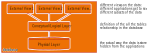
\includegraphics[width=0.85\linewidth]{\currentDir/threeSchemas}%
\caption{The Three-Schema Architecture of \glsreset{db}\pglspl{db}~\cite{AXSSGDMS1978FRODMS,TK1978TAXSDFROTSGODMS,BFJKMRGRT1985RMFDSDAFTGDOTAXSDSSG,SS2005EIDDDFDB:I}.}%
\label{fig:threeSchemas}%
\end{figure}

This means that a \pglspl{dbms} should support designing \pglspl{db} in the so-called three-schema architecture~\cite{AXSSGDMS1978FRODMS,TK1978TAXSDFROTSGODMS,BFJKMRGRT1985RMFDSDAFTGDOTAXSDSSG,SS2005EIDDDFDB:I} illustrated in \cref{fig:threeSchemas}:
It should be possible to provide different views on the data for different users and applications.
At the bottom layer of the \pgls{db} is the physical model managing how data is stored.
On top of that sits the conceptual~(or logical) layer, where the structure of the tables and the relationships between them are defined.
On the highest level, different views on the data can be provided for different applications.

In comparison, \microsoftExcel\ and \libreofficeCalc\ also offer us the ability to work with tables.
However, we cannot \emph{a priori} define a model or structure of the data that we want to store in tables.
While we can create some relations between cells of different tables, enforcing relationships on new rows that we are going to add is not possible.
While we can format cells and columns to emulate certain datatypes, we cannot strictly prevent that the user enters invalid data.
So these applications do not offer us any modeling capability on the logical level.
We have no influence on the way the data is stored and we cannot improve the performance by telling the applications to index the data in any reasonable way.
So there are no physical modeling capabilities either.
Finally, any person who would use a \microsoftExcel\ or \libreofficeCalc\ table as backend for different applications that have different views on data shall be stripped of their degree and credentials as a software developer.
Spreadsheets therefore obviously do not have any schema design capabilities at all and most certainly do not support anything resembling a three-schema architecture.
A \pgls{dbms} therefore needs to offer us data modeling tools that are very far beyond spreadsheets.%
\endhsection%
%
\hsection{Data Availability} %
The \pgls{dbms} makes a collection of data is available to users and applications in a meaningful format at a reasonable performance.
We expect that the speed of reading, writing, changing, deleting, and adding of data to the \pgls{db} be high.
A simple and reasonably abstract programming language should be provided for querying and updating the \pgls{db}.
There should also be tools available that further simplify the modeling, editing, and sorting of data as well as the generation of reports from data.%
\endhsection%
%
\hsection{Data Integrity}%
The correctness and validity of the data is ensured.
This includes several aspects:
First, the modeled relationships must be enforced.
If it is stated each bank account is associated with exactly one customer, then there must never be a bank account record that is not associated with an existing customer.
Also, there can never be two bank accounts with the same account~ID.
This property is called \emph{Consistency}.

Let's say that for each account, we store the current balance.
If a customer deposits money, then we can simply add the amount to their account's balance.
This is one operation where not much can ge wrong.
However, if money is transferred from one account of our bank to another account, then this \inQuotes{looks like} two operations.
But it actually is a single \emph{transaction}.
A \pgls{db} should be consistent before and after each transaction.

\emph{Atomicity} means that such a transaction will either complete successfully in its entirety or fail.
If the transaction is completed successfully, i.e., \emph{commits}, then all the changes become visible.
If the transaction is aborted, no change is performed.
No transaction can complete partially, it is all-or-nothing.
This means that either the money is correctly subtracted from one account and added to another \emph{or} nothing happens.
It must never happen that money is subtracted from one account but does not arrive in another due to an intermediate error.%
\endhsection%
%
\hsection{Concurrency Support and Isolation}%
Closely related to data integrity is the support for concurrency.
Multiple users and multiple processes can access and modify the \pgls{db} at the same time.
The \pgls{dbms} preserves the integrity of the \pgls{db} and of all the views that the users and process have on the data.

Different concurrent updates to the same account must take place atomically and in isolation.
This means that if money is transferred from account~$A$ to account~$B$ while simultaneously money is transferred from account~$B$ to account~$C$, the two transactions should not influence each other.
Both transactions should be isolated.

Another aspect of concurrency is that in some cases, we want to distribute databases over cluster of computers.
Maybe the databases are too big.
Maybe we want to increase the performance further by dividing the data into several sets which are almost independent.
Either way, an ideal \pgls{dbms} should offer us the functionality for doing that.%
\endhsection%
%
%
\hsection{Durability and Data Safety}%
A basic feature that any \pgls{db} needs to support is \emph{Durability}:
Once a transaction is committed, its changes are permanent.
The changes caused by the transaction are saved to the database permanently.

The \pgls{dbms} has to ensure that data can be preserved in case of unforeseen situations.
Indeed, durability extends also to system crashes and failures.
This includes the support of checkpoints and recovery after restarts.

Of course, there are limits to this:
At some lower layers, \pglspl{db} are stored as files in the filesystem.
If the underlying hard disk fails, these files can be destroyed.
There is no magical way a \pgls{dbms} can guard against this.
No system can be entirely safe from hard disk failures and crashes.

Therefore, \glspl{dbms} need to offer methods to back up the data, i.e., to create copies of the \pglspl{db} and store them on other devices.
Then, as long as reasonable backup strategies are employed, it must be possible to re-create the data after the original \pgls{db} was lost.
It is clear that for a bank, the data about its and its customers' accounts is its business.
If that data is lost, the bank is lost.
So ensuring that the database is robust and that it can be recreated from backups is of paramount importance.%
\endhsection%

The features \emph{A}tomicity, \emph{C}onsistency, \emph{I}solation, and \emph{D}urability together are often called \emph{ACID}~properties~\cite{GR1992TPCAT,WV2001TISTAATPOCCAR}.
%
\hsection{Data Privacy and Security}
\label{sec:featuresDataPrivacyAndSecurity}%
The \pgls{dbms} must enable the protection of data against access from unauthorized access from both within and outside of the organization.
It must be possible to specify roles for users and processes that define which data they can access or modify.
For example, the \pgls{dba} of the bank's \pgls{db} needs to be able to modify the structure of the \pgls{db}, maybe add and modify tables.
A normal bank employee should not be able to do that.
But they may be allowed to enter new records into certain tables of the the \pgls{db}, for instance, to add customers or to create new accounts.
Thinking this through even further, a bank employee may be assigned as manager to some customer's accounts.
The employees should only be able to see the information in these accounts.
All of this can be done by assigning roles to users and processes and access rights to roles.

The aforementioned three-schema architecture goes hand-in-hand with security measures.
At the highest level, the applications, users can only see the data that they need to be able to see and nothing more.
This is ensured by the different views that are provided for them.

Additionally, all access to the \pgls{db} should be password protected.
Communication with the \pgls{db} happens over encrypted connections.

A \pgls{dbms} should also support accounting and an audit trail.
It must be possible to log information regarding which user changed which dataset and when.
This is required to pass certain government, financial, or ISO certification audits.
\endhsection%
%
\hsection{Summary}%
It is quite obvious that the basic filesystem only offers very few of the properties discussed above.
Using simple data formats like \pgls{CSV} or even \microsoftExcel\ tables will not be a good choice either.
While one might realize concurrency by placing multiple interrelated such documents on a shared folder, there certainly would not be any \emph{ACID} guarantees.
Multiple people editing them at the same time will wreak havoc.
Structured formats like \pgls{JSON}, \pgls{XML}, or \pgls{YAML} would allow us to represent complex data in single documents, but this would make the multi-user access situation even worse.
And none of these solutions could provide any means to protect data integrity, let alone access control.

Instead, we require a software layer between the \pgls{db} and the user processes.
Honestly, we do not even really care of this software layer actually stores the data, how the data is organized internally, or how \emph{ACID} is implemented.
As long as this software, the \pgls{dbms}, offers us the above features, we will be happy.%
\endhsection%
\endhsection%
%
